\section{Identification of Cardinalities}

From these sentences in the specifications, we can also identify the cardinality of associations (one-to-one, one-to-many, many-to-many, etc.). For example, a treatment is administered during one or multiple races, and a team is funded by at least one sponsor.

\subsection{Association-Cardinality}
Identifying cardinalities is crucial to managing referential constraints between entities. These cardinalities determine which entity (table) should hold a reference (foreign key) to another entity (table) in an association or whether a new entity is required to link the two entities. This is especially necessary for many-to-many (M:N) relationships.

\begin{itemize}
\item \textbf{A} person \textbf{can be (but is not necessarily)} a rider, a sports director, or a soigneur.
\item \textbf{A} team consists of \textbf{multiple} riders.
\item \textbf{A} rider \textbf{may or may not} win stages.
\item \textbf{A} rider \textbf{may or may not} achieve rankings.
\item \textbf{A} stage results in \textbf{at least one} ranking.
\item \textbf{A} race consists of \textbf{at least one} stage.
\item \textbf{A} team \textbf{may or may not} win stages.
\item \textbf{Multiple} soigneurs provide treatment during \textbf{multiple} races.
\item \textbf{Multiple} soigneurs provide treatment at the request of \textbf{multiple} teams.
\item \textbf{Multiple} soigneurs administer \textbf{multiple} products.
\item \textbf{A} team \textbf{must have exactly} \textbf{one} sports director.
\item \textbf{A} team has \textbf{at least one} sponsor.
\end{itemize}

\subsection{UML Modeling (Version 1.2)}

Based on the identified cardinalities, we can propose a second version of the UML model.

\begin{figure}[H]
\begin{center}
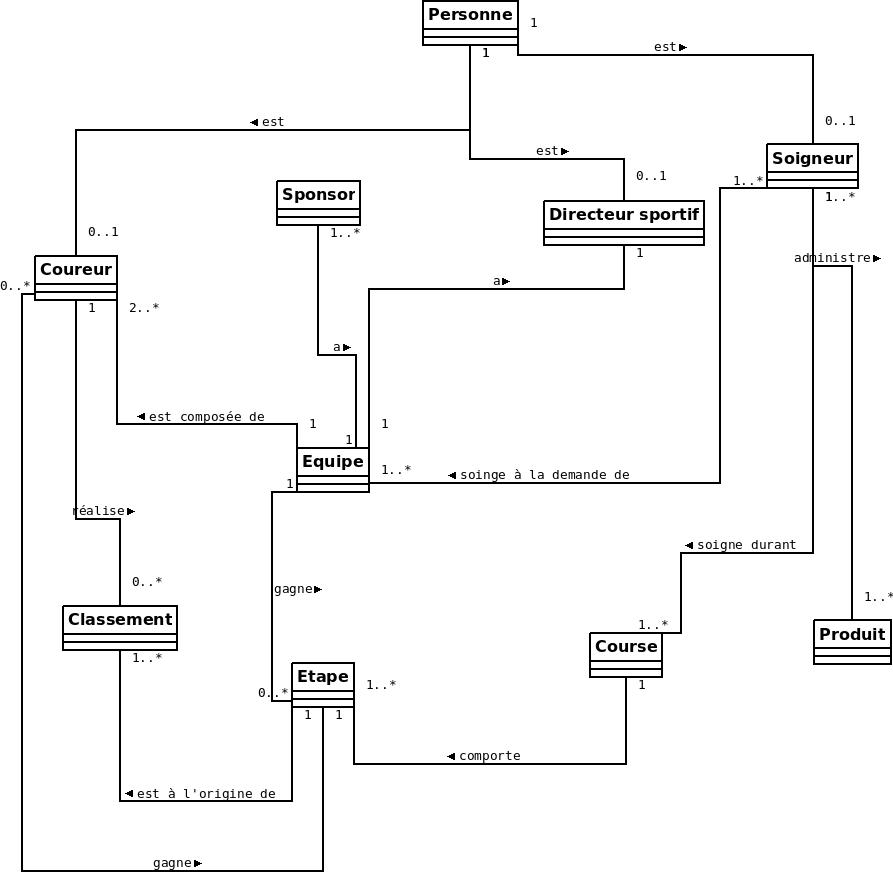
\includegraphics[height=7cm]{img/Figure2.jpg}\\
\caption{Model: Association Cardinalities}
\label{fig3}
\end{center}
\end{figure}

\newpage

\subsection{UML Modeling (Version 1.3)}
The previous UML model reveals several many-to-many relationships, which must systematically be broken down into two one-to-many associations. We can express this refinement more precisely by introducing associative tables (entities) and redefining the associations between these new tables and the two original entities.

First:
\begin{itemize}
\item \textbf{Multiple} soigneurs provide treatment during \textbf{multiple} races.
\end{itemize}
becomes:
\begin{itemize}
\item \textbf{A single} treatment is administered during \textbf{multiple} races.
\item \textbf{Multiple} soigneurs provide \textbf{a single} treatment.
\end{itemize}

Then:
\begin{itemize}
\item \textbf{Multiple} soigneurs provide treatment at the request of \textbf{multiple} teams.
\end{itemize}
becomes:
\begin{itemize}
\item \textbf{Multiple} soigneurs provide \textbf{a single} treatment.
\item \textbf{Multiple} teams receive \textbf{a single} treatment.
\end{itemize}

Finally:
\begin{itemize}
\item \textbf{Multiple} soigneurs administer \textbf{multiple} products.
\end{itemize}
becomes:
\begin{itemize}
\item \textbf{Multiple} soigneurs administer \textbf{a single} dose.
\item \textbf{Multiple} products are used within \textbf{the same} dose.
\end{itemize}

This results in the following model:

\begin{figure}[H]
\begin{center}
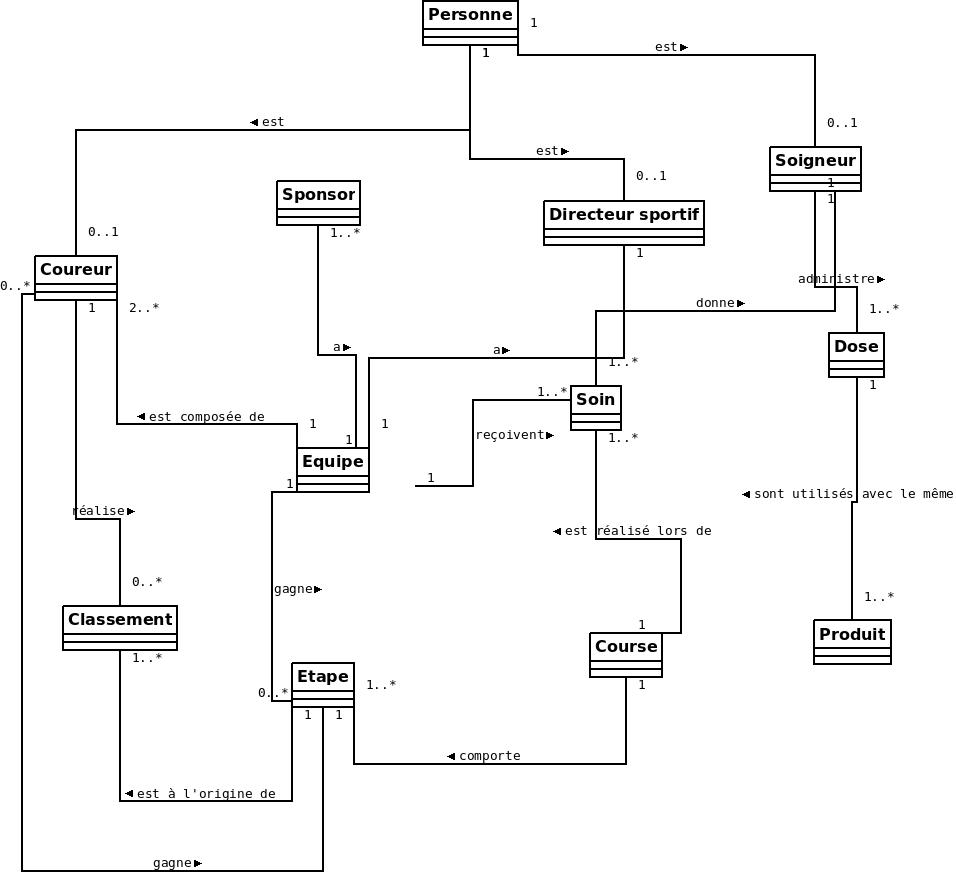
\includegraphics[height=7cm]{img/Figure3.jpg}\\
\caption{Model: Association Cardinalities}
\label{fig4}
\end{center}
\end{figure}
